%\documentclass{jsarticle}
%\documentclass[draft]
%\documentclass[dvipdfmx,autodetect-engine,draft]{jsarticle}% autodetect-engine で pLaTeX / upLaTeX を自動判定
\documentclass[dvipdfmx,autodetect-engine]{jsarticle}% autodetect-engine で pLaTeX / upLaTeX を自動判定

\usepackage[dvipdfmx]{graphicx}
\usepackage{url}
\usepackage{bm}
\usepackage{comment}
%\usepackage{split}
\usepackage{multirow}
\usepackage{listings,jlisting}
\usepackage{braket}
\usepackage{physics}
\usepackage{xparse,amsmath}
\usepackage{here}
\usepackage{enumerate}
\usepackage{mathrsfs}
%\usepackage{jlistings} %日本語のコメントアウトをする場合jlistingが必要
\setcounter{tocdepth}{3}
\usepackage{amsmath,amssymb}

\usepackage{empheq}



%ここからソースコードの表示に関する設定
\lstset{
  basicstyle={\ttfamily},
  identifierstyle={\small},
  commentstyle={\smallitshape},
  keywordstyle={\small\bfseries},
  ndkeywordstyle={\small},
  stringstyle={\small\ttfamily},
  frame={tb},
  breaklines=true,
  columns=[l]{fullflexible},
  numbers=left,
  xrightmargin=0zw,
  xleftmargin=3zw,
  numberstyle={\scriptsize},
  stepnumber=1,
  numbersep=1zw,
  lineskip=-0.5ex
}
\renewcommand{\lstlistingname}{ソースコード}
%ここまでソースコードの表示に関する設定

%
% proof environment without \qed
%
\makeatletter
%\renewenvironment{proof}[1][\proofname]{\par
\newenvironment{Proof}[1][\Proofname]{\par
  \normalfont
  \topsep6\p@\@plus6\p@ \trivlist
  \item[\hskip\labelsep{\bfseries #1}\@addpunct{\bfseries.}]\ignorespaces
}{%
  \endtrivlist
}
%\renewcommand{\proofname}{証明}
%\renewcommand{\proofname}{Proof}
\newcommand{\Proofname}{証明}
%\newcommand{\Proofname}{Proof}
\makeatother
%
% \qed
%
\makeatletter
\def\BOXSYMBOL{\RIfM@\bgroup\else$\bgroup\aftergroup$\fi
  \vcenter{\hrule\hbox{\vrule height.85em\kern.6em\vrule}\hrule}\egroup}
\makeatother
\newcommand{\BOX}{%
  \ifmmode\else\leavevmode\unskip\penalty9999\hbox{}\nobreak\hfill\fi
  \quad\hbox{\BOXSYMBOL}}
%\renewcommand\qed{\BOX}
\newcommand\QED{\BOX}



\begin{document}
%~~~~~~~~~~~~~~~~~~~~~~~~~~~~~~~~~~~~~~~~~~~~~~~~~~~~~~~~~~~


%分数
\newcommand{\f}[2]{\frac{#1}{#2}}
%偏微分ド(partial defferential)
\newcommand{\pd}[2]{\frac{\partial #1}{\partial#2}}
%微分
\newcommand{\D}[2]{\frac{ \mathrm{d} #1}{\mathrm{d}#2}}
%かける10のなんとか乗
\newcommand{\E}[1]{ \times 10^{#1}}
%数式中の単位(空白付き)
\newcommand{\un}[1]{~{\rm #1}}
%立体の添え字
\newcommand{\sub}[2]{#1_{\rm #2}}
%立体
\newcommand{\R}[1]{{\rm #1}}
%かける×
\def\*{\times}
%displaystyle
\newcommand{\dps}[1]{\displaystyle{#1}}
%ref
\newcommand{\rf}[1]{\ref{#1}}
%label
\newcommand{\lb}[1]{\label{#1}}
%\begin{equation}
\def\be{\begin{equation}}
%\end{equation}
\def\ee{\end{equation}}
%数式内の日本語
\newcommand{\jp}[1]{\mbox{#1}}
%イコールを揃える時の呪文
\def\bea{\begin{eqnarray}}
\def\eea{\end{eqnarray}}
%式番号をつけたくないときには
\def\bea*{\begin{eqnarray*}}
\def\eea*{\end{eqnarray*}}
%インテグラル
\newcommand{\I}[4]{\int_{#1}^{#2} \, #3 \, {\rm d} #4}
%レフト・ライト
\def\l{\left}
\def\r{\right}
%ベクトルの太文字 with \usepackage{bm}
%\newcommand{\vct}[1]{\bm{#1}}
%グラディエント
%\newcommand{\grad}[1]{{\rm grad}\, #1}
%ダイバージェント
%\newcommand{\Div}[1]{{\rm div}\, #1}
%ローテーション
%\newcommand{\rot}[1]{{\rm rot}\, #1}
%分散
%\def\var{{\rm var}}
%共分散
%\def\Cov{{\rm Cov}}
%平均のかっこ

\def\T{\mathsf{T}}

%~~~~~~~~~~~~~~~~~~~~~~~~~~~~~~~~~~~~~~~~~~~~~~~~~~~~~~~~~~~



\begin{flushright}
輪行予定日:2019年10月28日
\\慶應義塾大学理工学部物理学科\\岡崎健人
\end{flushright}
\begin{center}
{\Large Ridge回帰の実装} 
\end{center}
%箇条書き
%\tableofcontents   %👈目次
%\newpage


正則化パラメータ$\lambda$の値によって推定される曲線がどのように変わるのか、Fortran90でプログラムを組んで実験した。ここでは正則化項を$\lambda \norm{\vb*{w}}_2^2$とした(Ridge回帰)。

\section{正則化最小二乗法(Ridge回帰)}
トレーニングデータを$(x_i,y_i)_{i=1,\ldots,m}$と与える。これを$n$次関数$\hat{y}=w_0+w_1 x + w_2 x^2 + \cdots + w_{n} x^{n}=\displaystyle\sum_{k=0}^{n} w_k x^{k}$で近似する。$x$の次数順に並べたベクトルを$\vb*{x}=\qty[1,x,x^2,\ldots,x^{n}]^\mathsf{T},~$係数を並べたベクトルを$\vb*{w}=\qty[w_0,w_1,\ldots,w_{n}]^\mathsf{T}$とすれば(これらは$n+1$次の列ベクトル)、この関数は$\hat{y}=\vb*{w}^\mathsf{T} \vb*{x}$となる。各トレーニングデータ$(x_i,y_i)$を使って単純にこの$n$次多項式を計算した$\hat{y}_i=\displaystyle\sum_{k=0}^{n} w_k x_{i}^{k}$を並べた$m$次列ベクトルを$\hat{\vb*{y}}=\qty[\hat{y}_1,\ldots,\hat{y}_m]^\mathsf{T}$とする。これは行ベクトル${\vb*{x}_i}^{\mathsf{T}} = \qty[1,{x_i},{x_i}^2,\ldots,{x_i}^{n}]$を縦に並べた行列
$$X=\mqty[ {\vb*{x}_1}^{\mathsf{T}} \\ {\vb*{x}_1}^{\mathsf{T}} \\ \vdots \\ {\vb*{x}_{m}}^{\mathsf{T}}]=\mqty[ 1 & x_1 & {x_1}^2 & \ldots & {x_1}^{n} \\ 1 & x_2 & {x_2}^2 & \ldots & {x_2}^{n} \\ & & \vdots & &  \\1 & x_{m} & {x_{m}}^2 & \ldots & {x_{m}}^{n} ]$$
を用いて$\hat{\vb*{y}}=X \vb*{w}$とかける。ただしこの$X$は$m\times\qty(n+1)$の行列である。平均二乗誤差$\mathrm{MSE}\qty(\vb*{w})$を行列で表現して展開すると
\begin{eqnarray*}
\mathrm{MSE}\qty(\vb*{w}) &=& \frac{1}{m} \sum_{i=1}^{m} \qty(\hat{y}_i - y_i)^2=\frac{1}{m} \norm{\hat{\vb*{y}} - \vb*{y}}_2^2 = \frac{1}{m} \norm{X\vb*{w}-\vb*{y}}_2^2 \\
&=& \frac{1}{m} \qty(X\vb*{w}-\vb*{y})^\mathsf{T} \qty(X\vb*{w}-\vb*{y}) = \frac{1}{m} \qty(\vb*{w}^\mathsf{T} X^\mathsf{T} - \vb*{y}^\mathsf{T}) \qty(X\vb*{w}-\vb*{y}) \\
&=& \frac{1}{m} \qty( \vb*{w}^\mathsf{T} X^\mathsf{T} X \vb*{w}- \vb*{y}^\mathsf{T} X \vb*{w} - \vb*{w}^\mathsf{T} X^\mathsf{T} \vb*{y} +\vb*{y}^\mathsf{T} \vb*{y} )
\end{eqnarray*}
となる。ただし$\vb*{y}=\qty[y_1,\ldots,y_m]^\mathsf{T}$とした。目下の目的は平均二乗誤差$\mathrm{MSE}\qty(\vb*{w})$を最小化する$\vb*{w}$を求めることである。行列の微分の公式
$$\pdv{\vb*{w}}\qty(\vb*{w}^\mathsf{T} D \vb*{w})=\qty(D+D^\mathsf{T})\vb*{w},~~~\pdv{\vb*{w}}\qty(\vb*{a}^\mathsf{T} \vb*{w})=\pdv{\vb*{w}}\qty(\vb*{w}^\mathsf{T} \vb*{a})=\vb*{a}$$
を用いて平均二乗誤差$\mathrm{MSE}\qty(\vb*{w})$を微分すると
$$\pdv{\mathrm{MSE}\qty(\vb*{w})}{\vb*{w}} = \frac{2}{m} \qty(X^\mathsf{T} X  \vb*{w} - X^\mathsf{T} \vb*{y})$$
となるので、これが$\vb*{0}$となるのは$\vb*{w}=\qty(X^\mathsf{T} X)^{-1} X^\mathsf{T} \vb*{y}$のときである。\\


つぎに平均二乗誤差$\mathrm{MSE}\qty(\vb*{w})$を最小化するのではなく、重み減衰$\lambda\norm{\vb*{w}}_2^2=\lambda \vb*{w}^\T \vb*{w}$を加えたもの$J(\vb*{w})=\mathrm{MSE}\qty(\vb*{w}) + \lambda \vb*{w}^\T \vb*{w}$を最小化することを考える。$\pdv*{(\vb*{w}^\T \vb*{w})}{\vb*{w}}=2\vb*{w}$より
$$\pdv{J(\vb*{w})}{\vb*{w}}=\pdv{\mathrm{MSE}(\vb*{w})}{\vb*{w}}+\pdv{\qty(\lambda \vb*{w}^\T \vb*{w} )}{\vb*{w}}= \frac{2}{m} \qty(X^\mathsf{T} X \vb*{w} - X^\mathsf{T} \vb*{y}) + 2\lambda \vb*{w},$$
したがってこれが$\vb*{0}$となるのは
$\vb*{w}=\qty(X^\mathsf{T} X +m \lambda I)^{-1} X^\mathsf{T} \vb*{y}$
のときである。\\

プログラムを書くにあたって記号をいろいろ定義する。$A:=X^\T X,~B:=A+m\lambda I,~\vb*{v}:=X^\T\vb*{y}$とおく。すると目的は$(n+1)$本の1次連立方程式$B\vb*{w}=\vb*{v}$を$\vb*{w}$について解くことに帰着される。この目的は、さらに拡大係数行列$C:=\mqty[B&\vb*{v}]$にガウスの掃き出し法を行うことに帰着される。
ただし
$$X^\T = \mqty[1 & 1 & \cdots &1 \\ x_1 & x_2 & \cdots & x_m \\ {x_1}^2 & {x_2}^2 & \cdots & {x_m}^2 \\ \vdots & \vdots & & \vdots \\ {x_1}^n & {x_2}^n & \cdots & {x_m}^n],~~~X=\mqty[ 1 & x_1 & {x_1}^2 & \ldots & {x_1}^{n} \\ 1 & x_2 & {x_2}^2 & \ldots & {x_2}^{n} \\ & & \vdots & &  \\1 & x_{m} & {x_{m}}^2 & \ldots & {x_{m}}^{n} ]$$
より$A$の成分を具体的に書くと
$$A=X^\T X = \mqty[ s_0 & s_1 & s_2 & \cdots & s_m \\ s_1 & s_2 & s_3 & \cdots & s_{n+1} \\ s_2 & s_3 & \cdots & \cdots & s_{n+2}  \\ \vdots & \vdots & \ddots & \ddots & \vdots \\ s_n & s_{n+1} & s_{n+2} & \cdots & s_{n+n}],~~~~s_k=\sum_{i=1}^{m} {x_i}^k,~~~~k=0,\ldots,2n$$
となる。つまり$A$は対角線に垂直な方向の成分がすべて同じであるような、$(n+1)$次の対角行列になっている。その成分は$a_{ij}=s_{i+j-2},~i,j=1,\ldots,n+1$と定式化できる。$B$はその対角成分に$m\lambda$を加えた行列である。ただし$\lambda$は任意の変数であるから、$m\lambda$ではなく単に$\lambda$を加えることにする。
$$b_{ij}=\left\{\begin{array}{ll}{a_{ij}+ \lambda,} & {\mathrm{if}~i=j,} \\ {a_{ij},} & {\mathrm{if}~i\neq j.}\end{array}\right.$$
さらに$\vb*{v}$を具体的に示すと
$$\vb*{v}=X^\T \vb*{y} = \mqty[1 & 1 & \cdots &1 \\ x_1 & x_2 & \cdots & x_m \\ {x_1}^2 & {x_2}^2 & \cdots & {x_m}^2 \\ \vdots & \vdots & & \vdots \\ {x_1}^n & {x_2}^n & \cdots & {x_m}^n] \mqty[y_1 \\ y_2 \\ \vdots \\ y_m ] = \mqty[ v_0 \\ v_1 \\ \vdots \\ v_{n}],~~~~v_l = \sum_{i=1}^{m} {x_i}^{l} y_i,~~~~l=0,\ldots,n$$
である。拡大係数行列$C$は
\begin{equation}
C=\mqty[B & \vb*{v}]=\mqty[ b_{11} & b_{21} & \cdots & b_{n+1,1} & v_0 \\ b_{12} & \ddots & & \vdots & v_1 \\ \vdots & & \ddots & \vdots & \vdots \\ b_{1, n+1} & \cdots & \cdots & b_{n+1, n+1} & v_n] \label{C}
\end{equation}
よりその成分$c_{ij},~i=1,\ldots,n+1,~ j=1,\ldots,n+2$は
$$c_{ij}=\left\{\begin{array}{ll}{b_{ij},} & {\mathrm{for}~i,j=1,\ldots,n+1,} \\ {v_{i-1},} & {\mathrm{for}~i=1,\ldots,n+1,~j=n+2}\end{array}\right.$$
とかける。これは$(n+1)\times(n+2)$の行列になる。

\section{実験方法とソースコード}
まずデータを読み込んで、推定したい多項式の係数$\vb*{w} = \qty[w_0,\ldots,w_n]^\T$と、推定曲線の$(x,y)$の値を出力するプログラムを作成した。それをソースコード\ref{ridge}に示す。$\vb*{w} = \qty[w_0,\ldots,w_n]^\T$を求めるのには、式(\ref{C})の拡大係数行列$C$にガウスの消去法を適用した。データの数$m,~$多項式の次数$n,~$正則化パラメータ$\lambda,~$プロットの分割幅はプログラム作成者が入力できるようにした。$m$個の訓練データは、区間$[0,2)$の一様乱数を関数$2\cos\qty(2x)+x$に足すことで生成した。それをソースコード\ref{data_generator}に示す。

正則化パラメータを$\lambda = 10^4,~10^2,~10^0,~10^{-2},~10^{-4},~0$としたときに、$m=30$個のデータを$n=10,~20,~30$次の多項式で推定した。

\begin{lstlisting}[caption=リッジ回帰のソースコード,label=ridge]
program ridge_regression
 implicit none

 real(8), allocatable :: x(:), y(:), data(:), s(:), v(:)
 real(8), allocatable :: a(:, :), b(:, :), c(:, :), w(:)
 real(8) :: lambda, p, q, width, delta, xmin, y_hat, x1
 integer :: i, j, n, m, k, l, i1, i2

 ! ***入力*********************
   ! データの数
   m = 30

   ! 近似したい曲線の次数
   n = 10

   ! 正則化パラメータ
   lambda = 1.0_8

 !***データの読み込み***********************
  allocate(x(m), y(m), data(2 * m))
  ! mx2のデータ(「data.txt」など)をサイズ2mの配列data(2*m)として読み込む。
  ! (「./a.out < data.txt」 )
  ! data(2*m)はx,y,x,y,…のような並びになっている。

  read(*,*) data

  ! data(2*m)の奇数番目をx(j), 偶数番目をy(j)とする。
  do i = 1, 2*m
    if ( mod(i, 2) == 0 ) then
      j = i / 2
      y(j) = data(i)
    else if ( mod(i, 2) == 1 ) then
      j = (i + 1) / 2
      x(j) = data(i)
    end if
  end do

! 確認済み
! do j = 1, m
!  write(*,*) j, x(j), y(j)
! end do

!***拡大係数行列の準備***********************************
! 解きたい連立方程式Bw=vのBとvの成分を計算しておく。
! 拡大係数行列C=[B v]を構築する。
  allocate(s(0:2 * n), a(n + 1, n + 1), b(n + 1, n + 1), v(0 : n), c(n + 1,  n + 2))

! s_k = sum_{i=1}^{m} {x_i}^k, k=0~2nの計算
  do k = 0, 2 * n
    s(k) = 0.0_8
    do i = 1, m
      s(k) = s(k) + (x(i)) ** (real(k))
    end do
!    write(*,*) k, s(k)
  end do

  ! 行列Aの計算。その成分はa_{ij}=s_{i+j-2}, i,j=1~n+1.
  do j = 1, n + 1
    do i = 1, n + 1
      a(i, j) = s(i + j - 2)
  !    write(*,*) i, j, i + j - 2, s(i + j - 2), a(i, j)  ! 確認済み
    end do
  end do

  ! 行列Bの計算。行列Aの対角成分にlambdaを足すだけ。
  do j = 1, n + 1
    do i = 1, n + 1
      if ( i == j ) then
        b(i, j) = a(i, j) + lambda
      else if ( i /= j ) then
        b(i, j) = a(i, j)
      end if
!      write(*,*) i, j, b(i, j) - a(i, j) ! 確認済み。
    end do
  end do

! v_l = sum_{i=1}^{m} y_i {x_i}^l, l=0~nの計算
   do l = 0, n
     v(l) = 0.0_8
     do i = 1, m
       v(l) = v(l) + y(i) * (x(i)) ** real(l)
     end do
!     write(*,*) l, v(l) ! 確認済み
   end do

! 拡大係数行列C=[B v]を作る
  do i = 0, n
    do j = 1, n + 2
      if (j == n + 2) then
        c(i + 1, j) = v(i)
      else if (j /= n + 2) then
        c(i + 1, j) = b(i + 1, j)
      end if
    end do
  end do
!   確認済み
!  do i = 0, n
!    do j = 1, n + 2
!      write(*,*) i + 1, j, v(i), c(i + 1, j)
!    end do
!  end do

! ***ガウスの掃き出し法**************************************
! 上で作った(n+1)x(n+2)の拡大係数行列Cにガウスの掃き出し法を適用する。
! あるk行目の対角成分c(k,k)をpとおき、その行すべてをpで割る。
! そうすればその対角成分c(k,k)は1になる。
! k行目以外の行について(これをi行目とする)、c(k,k)と同じ列にあるもの(c(i,k))をqとおく。
! そのi行目のk列目以降の成分c(i,j), j=k~n+2 からq*c(k,j)を引く。
! これでc(k,k)の上下はゼロになる。
! このことをすべての行 k=1~n+1 について行う。

  do k = 1, n + 1
    p = c(k, k)
    do j = k, n + 2
      c(k, j) = c(k, j) / p
    end do
    do i = 1, n + 1
      if (i /= k) then
        q = c(i, k)
        do j = k, n + 2
          c(i, j) = c(i, j) - q * c(k, j)
        end do
      end if
    end do
  end do

!   確認済み
!   do i = 1, n + 1
!     do j = 1, n + 2
!       write(*,*) i, j, c(i, j)
!     end do
!   end do

! こうして得られた行列の最後の列c(i,n+2), i=1~n+1がwの解である。
  allocate(w(n + 1))
    do i = 1, n + 1
      w(i) = c(i, n + 2)
      write(*,*)  i - 1, w(i) ! 確認済み
    end do

! ***曲線のプロット****************************************
! 分割数
  i1 = 200

! xの幅widthとxの最小値xminを計算。
  width = maxval(x) - minval(x)
  xmin = minval(x)
!    write(*,*) width, xmin, maxval(x) ! 確認済み

  ! 曲線のプロットの刻み幅
  delta = width / real( i1 )

  open (18, file='line.txt', status='replace')
  do i2 = 0, i1
    y_hat = 0.0_8
    x1 = xmin + real(i2) * delta
      do i = 1, n + 1
        y_hat = y_hat + w(i) * x1 ** (real(i - 1))
      end do
    write(18, *) x1, y_hat ! ここでxに対する近似曲線y_hat=sum_{k=0}^{n} w_k x^kの値を出力
  end do
  close(18)

  deallocate(x, y, data, s, v, a, b, c, w)

 stop
end program
\end{lstlisting}

\begin{lstlisting}[caption=データ生成のためのプログラム,label=data_generator]
program data_generator
 implicit none

 integer :: m, imax, i
 real(8) :: xmin, xmax, width, delta, x, y
 real(8), allocatable :: random(:)


! データの個数
  m = 30

  allocate(random(m + 1))
  call random_number(random)
  ! 確認
!  do i = 0, m
!   write(*,*) i, 2.0_8 * random(i + 1)
!  end do

! データの最小値・最大値の設定、幅、分割幅
  xmin = 0.0_8
  xmax = 6.0_8
  width = xmax - xmin
  delta = width / real(m)
!  write(*,*) width

  open(18, file='generated_data.txt', status='replace')
  do i = 0, m - 1
    x = xmin + delta * real(i)
    y = 2.0_8 * cos(2.0_8 * x) + x  + 2.0_8 * random(i + 1)
    write(18,*) x, y
  end do
  close(18)

  deallocate(random)
  
  stop
 end program
\end{lstlisting}


\section{出力結果}
$n=10,~20,~30$に対して正則化パラメータを$\lambda = 10^4,~10^2,~10^0,~10^{-2},~10^{-4},~0$としたときの推定結果を図\ref{10_big}から図\ref{30_small}に示す。与えた30個のデータは点で表し、推定した曲線を実線で表している。ただし推定した曲線は$200$個の点を線で繋いだものなので、鋭いピークがあるとそれが削れてい表示されている可能性がある。

$n=10$など$n$が比較的小さいとき、$\lambda$の値が大きいときちんとデータ点を推定しておらず、過少適合をおこしているのが観察できる。逆に$n=30$など$n$が大きく$\lambda$が小さいときには過剰適合を起こしている。

$n=30,~\lambda = 10^2$のときの推定曲線が過剰に振動している。$\lambda$の値を少し変えて$\lambda=99,101$として比較したが、そのようなことは起こっていなかった(図\ref{99100101})。なぜそうなるのかはよくわからない。   



%2枚の図
\begin{figure}[htbp]
 \begin{minipage}{0.5\hsize}
  \begin{center}
   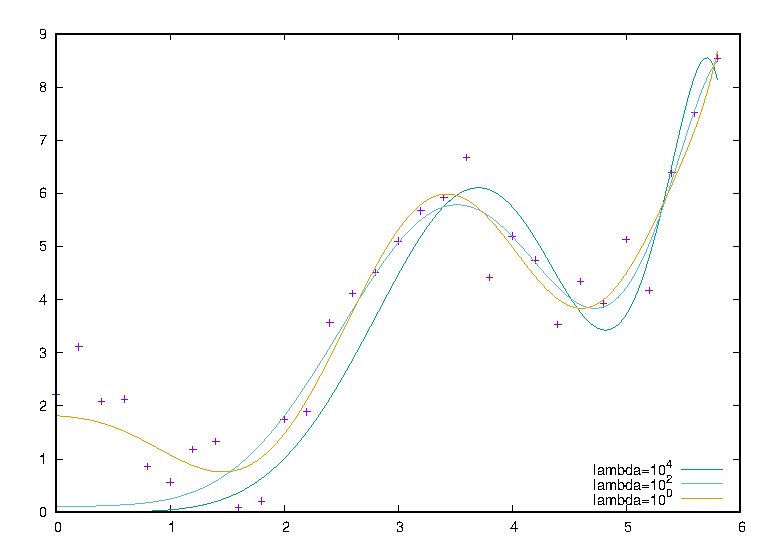
\includegraphics[width=70mm]{10_big.eps}
  \end{center}
  \caption{$n=10,~\lambda = 10^4,10^2,~0^0$}
  \label{10_big}
 \end{minipage}
 \begin{minipage}{0.5\hsize}
  \begin{center}
   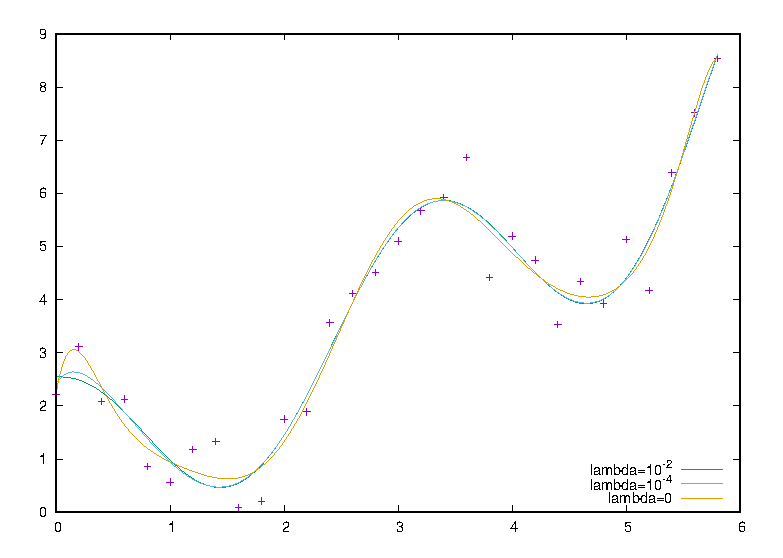
\includegraphics[width=70mm]{10_small.eps}
  \end{center}
  \caption{$n=10,~\lambda = 10^{-2},10^{-4},0$}
  \label{10_small}
 \end{minipage}
\end{figure}

%2枚の図
\begin{figure}[htbp]
 \begin{minipage}{0.5\hsize}
  \begin{center}
   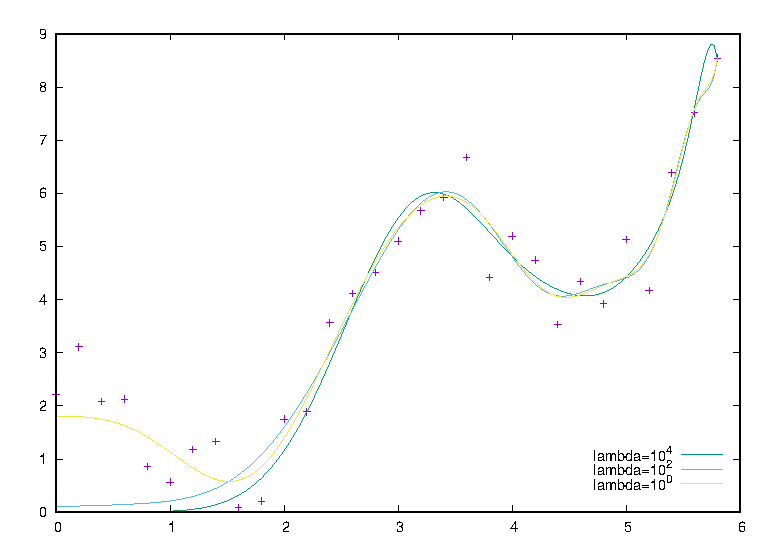
\includegraphics[width=70mm]{20_big.eps}
  \end{center}
  \caption{$n=20,~\lambda = 10^4,10^2,10^0$}
  \label{}
 \end{minipage}
 \begin{minipage}{0.5\hsize}
  \begin{center}
   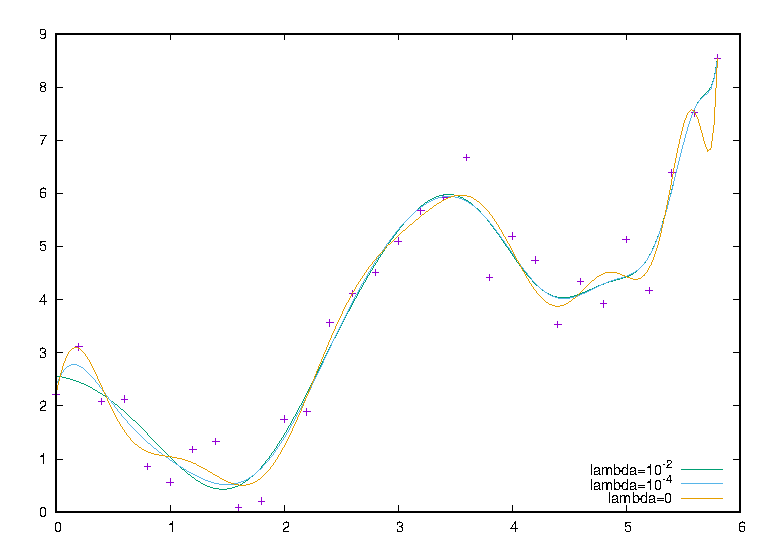
\includegraphics[width=70mm]{20_small.eps}
  \end{center}
  \caption{$n=20,~\lambda = 10^{-2},10^{-4},0$}
  \label{}
 \end{minipage}
\end{figure}

%2枚の図
\begin{figure}[htbp]
 \begin{minipage}{0.5\hsize}
  \begin{center}
   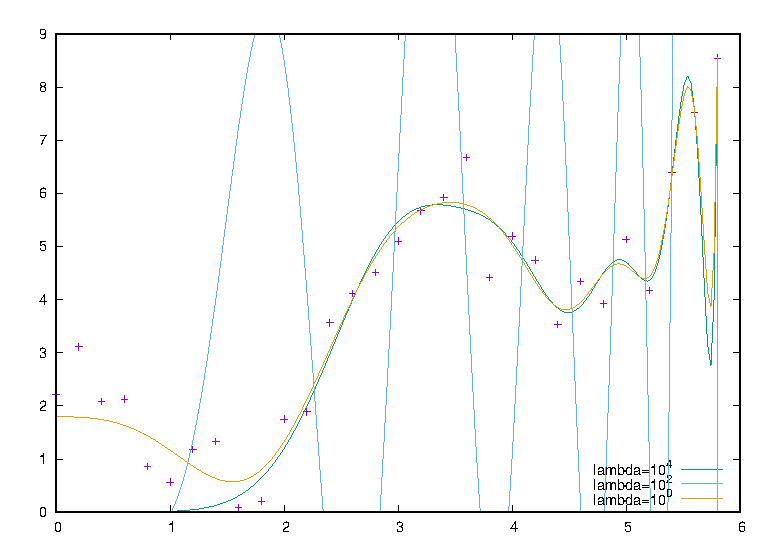
\includegraphics[width=70mm]{30_big.eps}
  \end{center}
  \caption{$n=30,~\lambda = 10^4,10^2,10^0$}
  \label{}
 \end{minipage}
 \begin{minipage}{0.5\hsize}
  \begin{center}
   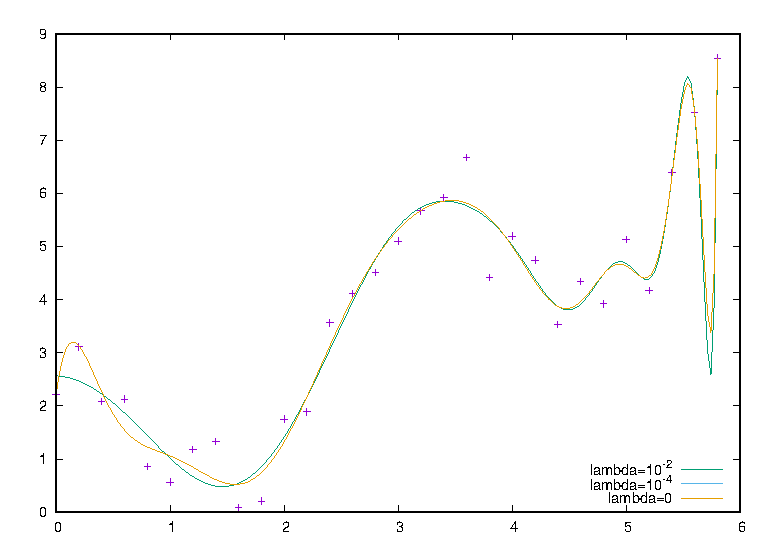
\includegraphics[width=70mm]{30_small.eps}
  \end{center}
  \caption{$n=30,~\lambda = 10^{-2},10^{-4},0$}
  \label{30_small}
 \end{minipage}
\end{figure}

%1枚の画像
\begin{figure}[htbp]
\centering 
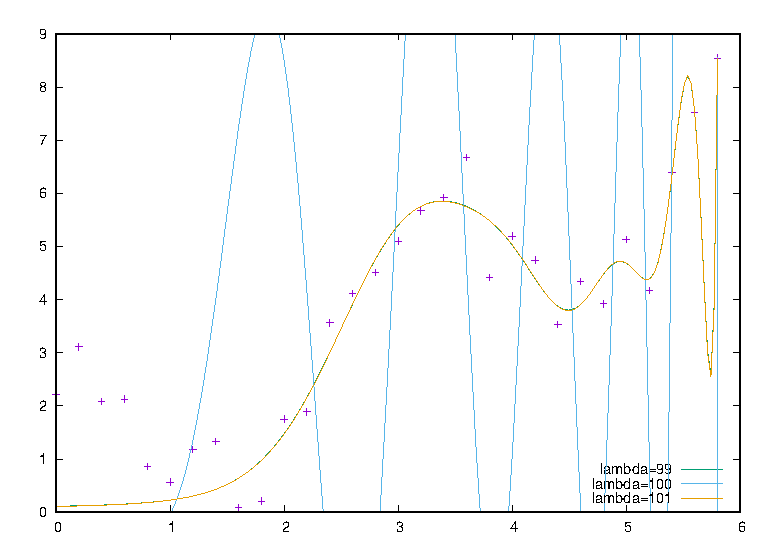
\includegraphics[width=120mm]{99100101.eps}
\caption{$n=30$のときに$\lambda = 99,100,101$を比較したもの}
\label{99100101}
\end{figure}


\section{今後の課題}
なぜ$n=30,~\lambda = 10^2$のときに異常な出力を得たのかを解決したい。

また適切な$n$と$\lambda$をどう決めるのかわからなかった。そこで$n$と$\lambda$を少しづつ変えて出力させ、テストデータを与えて汎化誤差が一番小さい$n$と$\lambda$を適切なものとする、というようなプログラムも書けるだろう。






%\begin{thebibliography}{9}
%  \bibitem{進化論的計算手法} 伊藤斉志,「進化論的計算手法」,2005年.pp. 107--122.
%\end{thebibliography}

\end{document}